\documentclass[12pt, twoside]{report}

%% comment this line for handouts. Uncomment for lecture notes
%\newcommand{\lectureNoteMode}{}

\raggedbottom

\usepackage{color, xifthen, amsthm, amssymb, amsmath, tikz, pgfplots}
\pgfplotsset{compat=1.18}
\usetikzlibrary{backgrounds}
\usepackage[letterpaper, margin=1in]{geometry}
\usepackage{multicol}
\usepackage{fourier}  %don't use txfonts b/c the sf doesn't look good

\usepackage{enumitem}
\setlist{topsep=-\parskip/2}


\setlength{\parindent}{0pt}
\setlength{\parskip}{\baselineskip}


\usepackage{mdframed} % makes better frames around examples (eg pagebreak allowed)
  % from mdframed package. used for examples
\newmdenv[
  skipabove=10pt,%\topsep,
  skipbelow=10pt,%\topsep
  ]{allrules}

\usepackage{tcolorbox} % for colored boxes


\usepackage{subfigure}
\usepackage{hyperref}
\hypersetup{colorlinks, urlcolor=red, linkcolor=.} %color urls, but not interal refs
\usepackage{graphicx, floatflt}
\graphicspath{{./figs/}{../figs/}}
\DeclareGraphicsExtensions{.png,.jpg,.pdf}

\usepackage{wrapfig}  %useful for wrapping text around pictures or tables
		      %though it doesn't do a great job inside my example boxes


\definecolor{defbod}{rgb}{.8,.8,.8}     \definecolor{defhead}{rgb}{.7,.1,.1}
\definecolor{thmbod}{rgb}{.8,.8,.8}     \definecolor{thmhead}{rgb}{.1,.1,.9}
\definecolor{factbod}{rgb}{1,1,1}    \definecolor{facthead}{rgb}{.1,.7,.1}
\definecolor{exbod}{rgb}{1,1,1}         \definecolor{exhead}{rgb}{0,.3,0}
\definecolor{soltext}{rgb}{.2,.2,.5}
\definecolor{notebod}{rgb}{.9,.9,.9}    \definecolor{notehead}{rgb}{.1,.1,.7}

\newcommand{\defn}[1]{
 \noindent \colorbox{defbod}{\begin{minipage}{.95\linewidth}
 \hspace{-12pt}\colorbox{defhead}{\sf\color{white} Definition}
 #1
 \end{minipage} } \medskip
 }
\newcommand{\dt}[1]{\textcolor{defhead}{\bfseries #1}}

\newcommand{\thrm}[1]{
 \noindent \colorbox{thmbod}{\begin{minipage}{.95\linewidth}
 \hspace{-12pt}\colorbox{thmhead}{\sf\color{white}Theorem}
 #1
 \end{minipage} } \medskip
 }
\newcommand{\coro}[1]{
 \noindent \colorbox{thmbod}{\begin{minipage}{.95\linewidth}
 \hspace{-12pt}\colorbox{thmhead}{\sf\color{white}Corollary}
 #1
 \end{minipage} } \medskip
 }
\newcommand{\fact}[1]{  %%%% !! note this different from calcnotes
 \noindent \begin{allrules}
 #1
 \end{allrules} \medskip
 }

\newcommand{\note}[1]{
	\noindent \colorbox{notebod}{\begin{minipage}{.95\textwidth}
			\hspace{-12pt}\colorbox{notehead}{\sf\color{white}NOTE}
			#1
	\end{minipage} } \medskip
}


% making the example thing with a line down the left.
\newmdenv[
rightline=false,
bottomline=false,
skipabove=0pt,%\topsep,
skipbelow=0pt,%\topsep
]{siderules}

\newcommand{\ex}[1]{
  \noindent \begin{siderules}
    \textcolor{exhead}{\sf Example}
    #1
  \end{siderules} 
  \medskip
}




%%%%%%%%%% set it up so that these are not displayed when 
%%%%%%%%%% printing notes for students?  or for overhead?
\newcommand{\exsol}[1]{
  {\color{soltext} #1}
}

\newcommand{\mynonumsect}[2][]{
 \cleardoublepage
 \section*{#1\hskip16pt #2}
 \addcontentsline{toc}{section}{#1 #2}
}

\newcommand{\myhead}[1]{
\par%\vskip\baselineskip
\noindent
{\large\bf #1}
}

%%%%%%%%%%%%%%%%%%%%%%%%
% symbol shortcuts

\newcommand{\nice}{\displaystyle}
\newcommand{\eqq}{\ensuremath \stackrel{?}{=}}
\newcommand{\R}{\ensuremath{\mathbb{R}}}




% %%%%%%%%%%%%%%%%%%%%%%%%
% %
% % Creating handouts vs notes
% %% If you use the line below before loading this file then it will be set up for
% %% lecture notes.  Default is for handouts
% %%
% %% \newcommand{\lectureNoteMode}{}
% %%
% %% do not uncomment here, just add the line to the file where you input this one.
% \ifthenelse{\not\isundefined\lectureNoteMode}
% { % lecture notes 
%   \newcommand{\Hvskip}[1]{}
%   \newcommand{\Hvfill}{}
%   \newcommand{\Hpbreak}{}  % pagebreaks for handouts
%   \newcommand{\Npbreak}{\vfill\pagebreak} % pagebreaks for printable notes
%   \newcommand{\Nonly}[1]{#1} % shows in notes, not in handouts
%   \newcommand{\mycleardoublepage}{\cleardoublepage}

%   \newcommand{\ex}[1]{
%    \noindent \begin{allrules}
%     \textcolor{exhead}{\sf Example}\par
%     #1
%     \end{allrules} \medskip
%   }

% } 
% { 
% %% Handout mode 
% %% this section sets it up with smaller margins, and blank spots for writing solns to examples
%   %%%%%%%%%%%%%%%%%%%%%%%%%%%%%%%%%%%%%%%%%%
%   %change frame around examples
%   % from mdframed package
%   \newmdenv[
%   rightline=false,
%   bottomline=false,
%   skipabove=0pt,%\topsep,
%   skipbelow=0pt,%\topsep
%   ]{siderules}
  
%   \newcommand{\ex}[1]{
%     \noindent \begin{siderules}
%       \textcolor{exhead}{\sf Example}
%       #1
%     \end{siderules} 
%     \medskip
%   }
  
%   %
%   %%%%%%%%%%%%%%%%%%%%%%%%%%%%%%%%%%%%%%%%%%
  
%   % don't show solutions for examples
%   \renewcommand{\exsol}[1]{}
  
%   %used for making blank space in handouts. eg: \vs2
%   \newcommand{\Hvskip}[1]{\vskip#1in\null}
%   \newcommand{\Hvfill}{\vfill} %vfill only in handouts mode
%   \newcommand{\Hpbreak}{\pagebreak} % pagebreaks for handouts
%   \newcommand{\Npbreak}{} % pagebreaks for printable notes
%   \newcommand{\Nonly}[1]{} % shows in printable, not in handouts
%   \newcommand{\mycleardoublepage}{\newpage} % don't need blank pages if not printing
  
%   % don't really need margins since not printing.
%   \geometry{margin=0.75in}

%   \renewcommand{\mynonumsect}[2][]{
%     \mycleardoublepage
%     \section*{#1\hskip16pt Handout: #2}
%     \addcontentsline{toc}{section}{#1 #2}
%   }

% } 





\setlength{\parindent}{0pt}

\setcounter{chapter}{1}
\begin{document}

\mynonumsect[1.5]{Graphs of Linear Functions}

\textbf{Goals:} 
\begin{itemize}
	\item To graph a line using slope, including horizontal and vertical lines
	\item To determine if two lines are parallel, perpendicular, or intersecting
	\item To find $x$-intercepts and $y$-intercepts, intersection points
\end{itemize}


\defn{\dt{Graphical Interpretation of a Linear Equation} \\
	
Graphically, in the equation $f(x) = mx+b$ \hskip0.25in (or alternatively, $f(x) = b +mx$), \\
	\begin{itemize}
		\item $b$ is the vertical intercept of the graph and tells us we can start our graph at $(0, b)$
		\item $m$ is the slope of the line and tells us how far to rise and run to get to the next point		
	\end{itemize}
\vskip6pt 	
Once we have at least 2 points, we can extend the graph of the line to the left and right.
}

\ex{Graph $f(x)= -\frac{2}{3}x +5$.
}
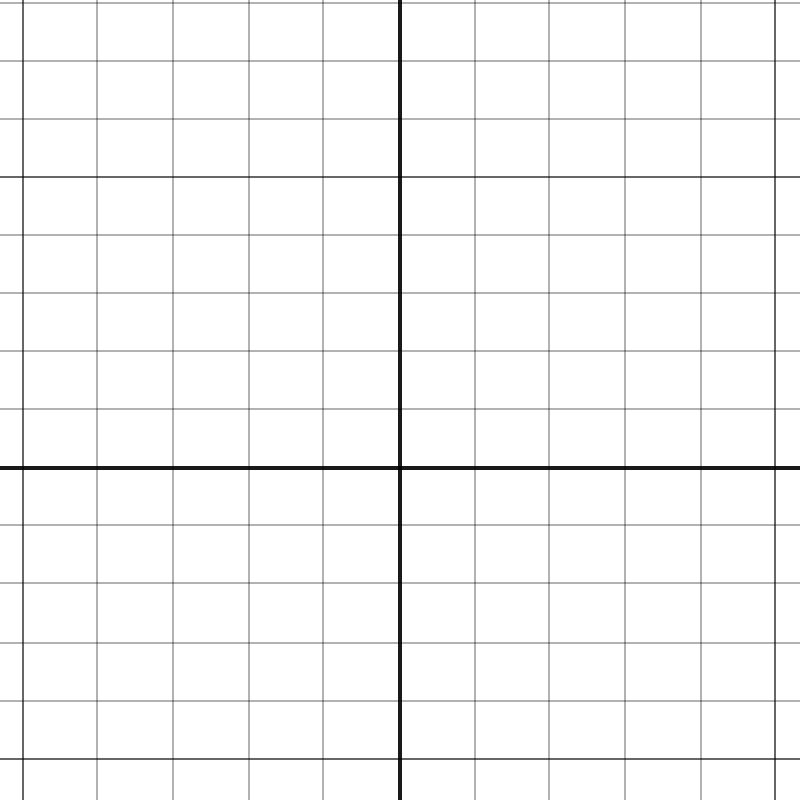
\includegraphics[alt={Blank graph paper for graphing the line f of x equals negative two thirds x plus five.}, width=4.5in]{105_graphpaper.jpg}

\pagebreak


\defn{\dt{Horizontal $y$-intercept} of the function is where the graph crosses the horizontal axis.  \\
If a function has a horizontal intercept, you can always find it by solving f(x) = 0.
}

\ex{
\begin{enumerate}
	\item Match each equation with one of the lines in the graph below.
	
	\begin{multicols}{2}
		\begin{itemize}
			\item $f(x)=2x+3$
			\item $g(x)=2x-3$
			\item $h(x)=-2x+3$
			\item $j(x)=\frac12 x+3$
		\end{itemize}
	\end{multicols}
	
	\item Find the horizontal $y$-intercept of each line algebraically.  Check with the graphs!
\end{enumerate}

}


\vfill 

\begin{center} 
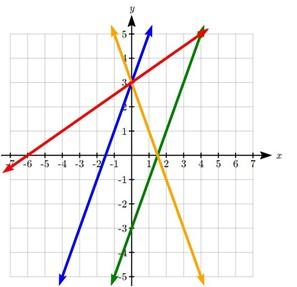
\includegraphics[alt={Coordinate plane showing four lines for matching equations and finding horizontal intercepts.}, width=3.5in]{105_1.5_figure1.jpg}
\end{center} 



\pagebreak

Find the $x$-intercept and the $y$-intercept, then plot.

\begin{enumerate}
	\item
	$y = - 3x + 3$ 
	\\ \phantom{.}\hfill
	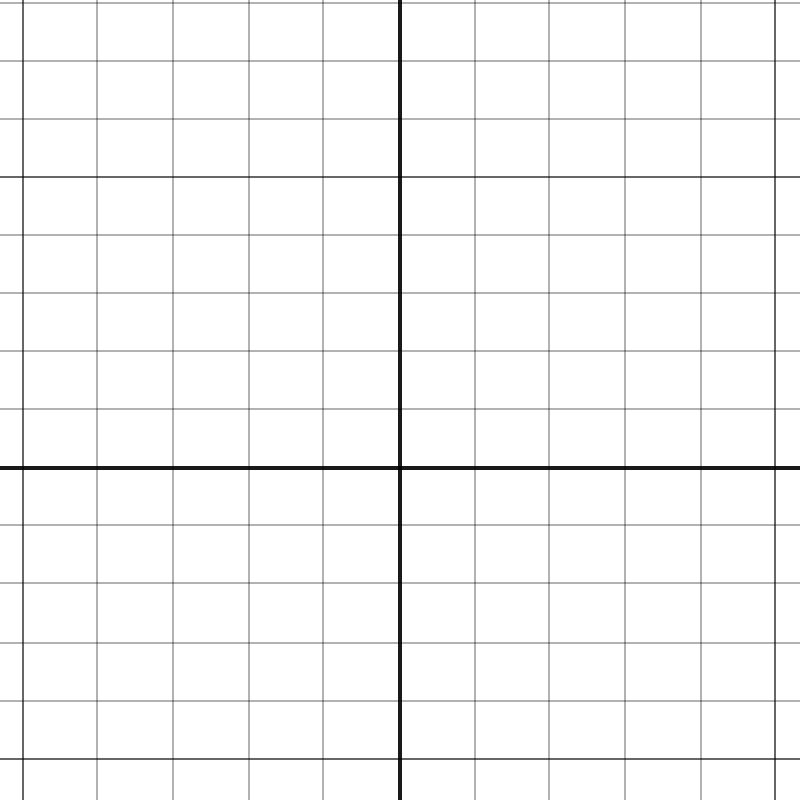
\includegraphics[alt={Blank graph paper for plotting the x-intercept and y-intercept of the given line.}, width=1.5in]{105_graphpaper.jpg}
	
	\item
	$y = - 2x - 2$
	\\ \phantom{.}\hfill
	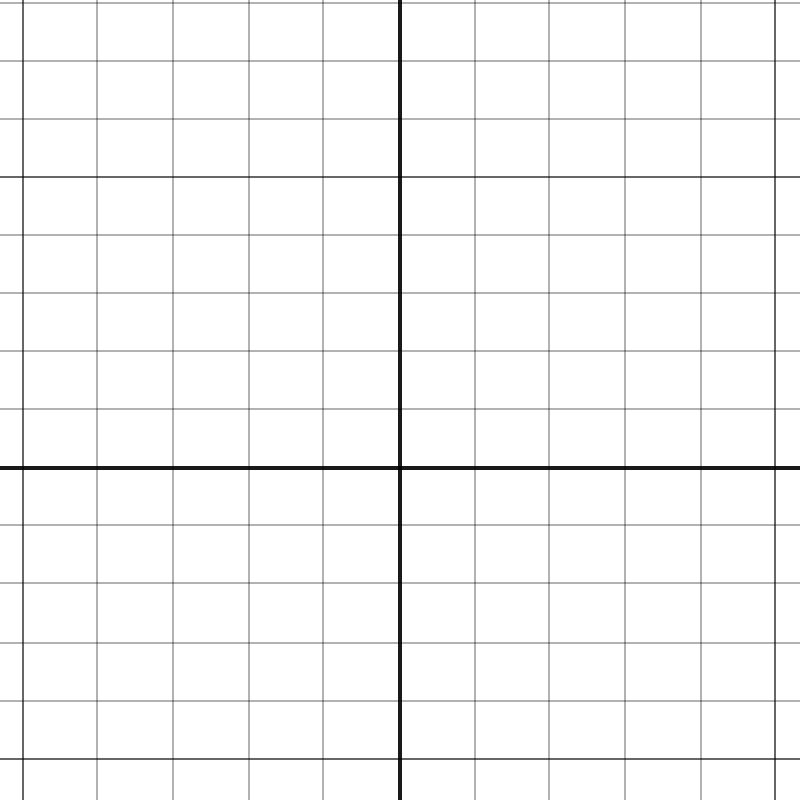
\includegraphics[alt={Blank graph paper for plotting the x-intercept and y-intercept of the given line.}, width=1.5in]{105_graphpaper.jpg}
	\item
	$y = \frac{1}{2}x - 1$
	\\ \phantom{.}\hfill
	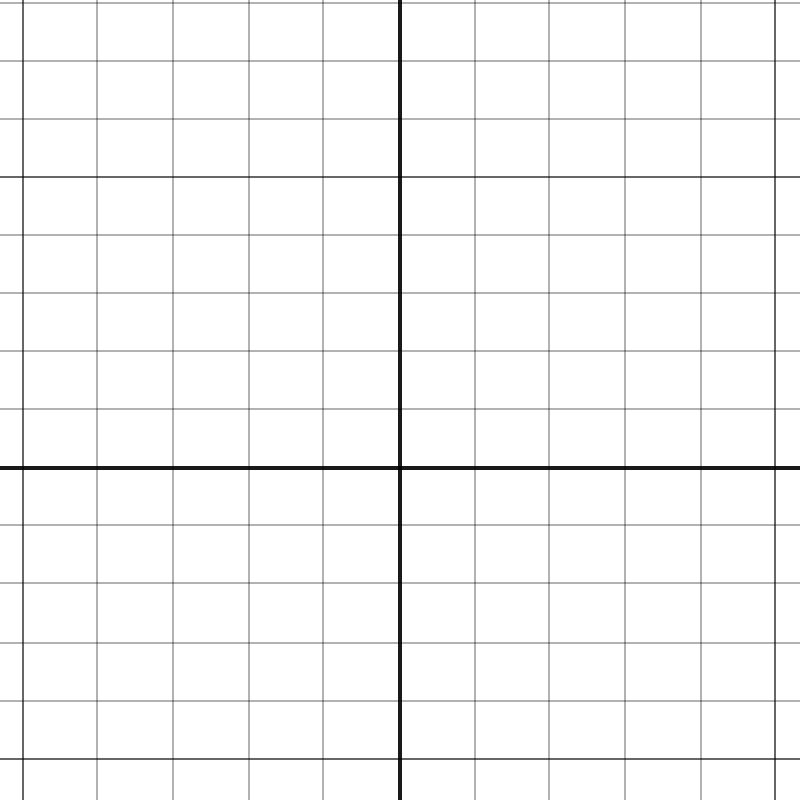
\includegraphics[alt={Blank graph paper for plotting the x-intercept and y-intercept of the given line.}, width=1.5in]{105_graphpaper.jpg}
	\item
	$x - 3y = - 3$ 
	\\ \phantom{.}\hfill
	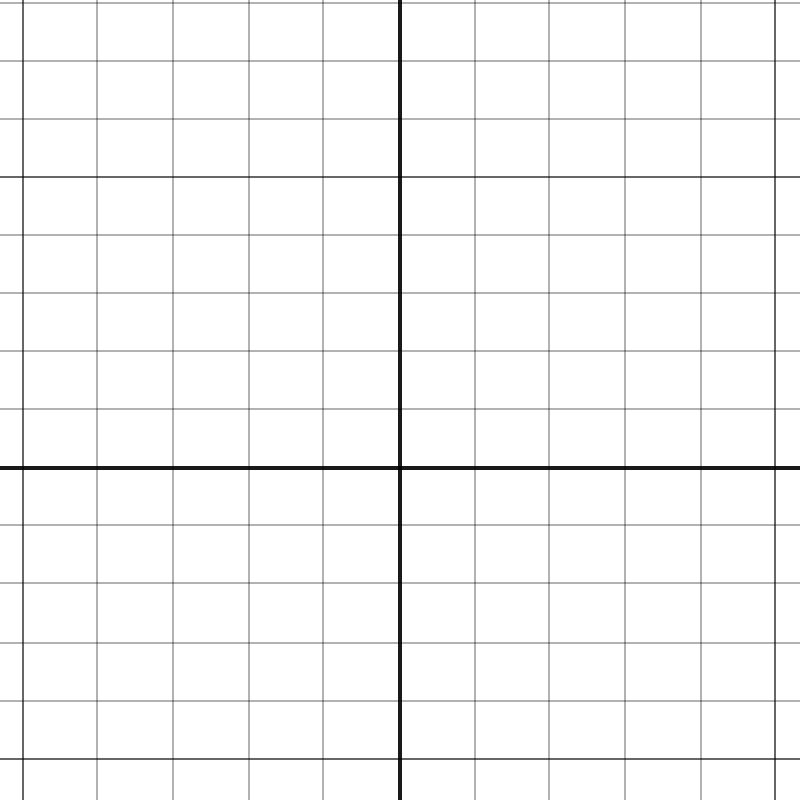
\includegraphics[alt={Blank graph paper for plotting the x-intercept and y-intercept of the given line.}, width=1.5in]{105_graphpaper.jpg}
\end{enumerate}




\pagebreak



\defn{\dt{Special Cases of Lines} \\
	
\begin{itemize}
	\item Horizontal Line: $y = b$, slope is zero. \\
	Has $y$-intercept: $(0,b)$ \\
	
	\item Vertical Line: $x = a$, slope is undefined. \\
	Has $x$-intercept: $(a,0)$ \\
\end{itemize}

}

Write the equation of the line in slope-intercept form with the given characteristics. Then plot.

\begin{enumerate}
\item
  A horizontal line that passes through the point $({-2,8})$. \\ \phantom{.}\hfill
  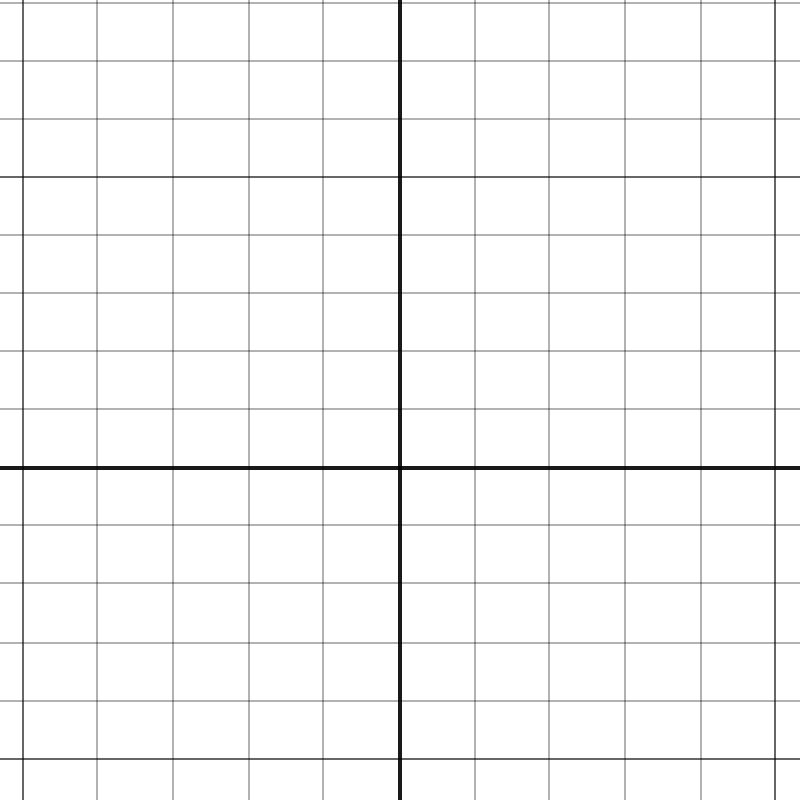
\includegraphics[alt={Blank graph paper for plotting the horizontal or vertical line described in the problem.}, width=1.25in]{105_graphpaper.jpg}

\item
  A horizontal line that passes through the point $({2, -5})$. \\ \phantom{.}\hfill
  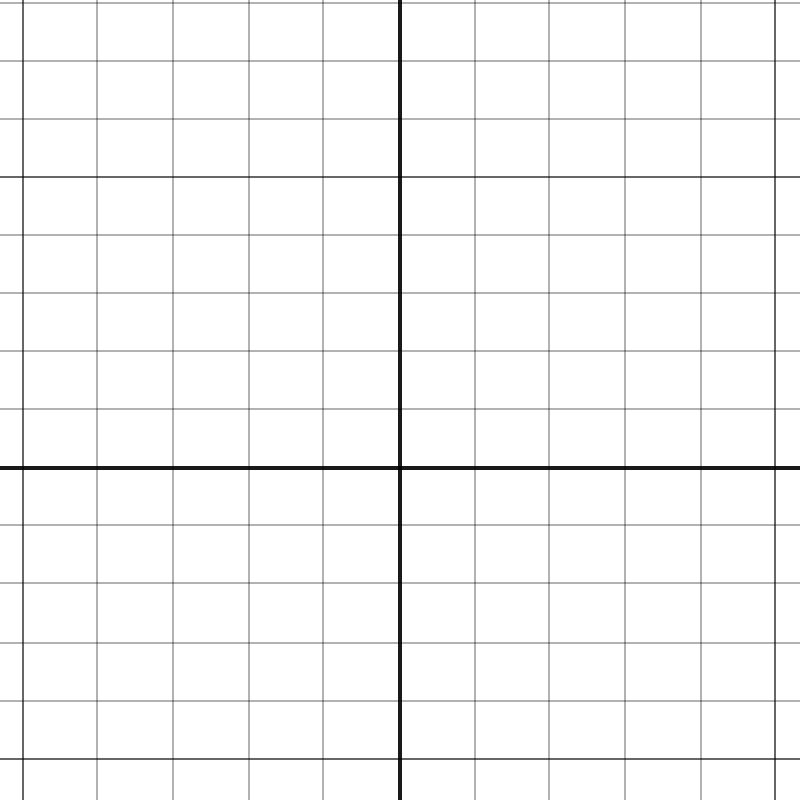
\includegraphics[alt={Blank graph paper for plotting the horizontal or vertical line described in the problem.}, width=1.25in]{105_graphpaper.jpg}
  
\item
  A vertical line that passes through the point $({-2,8})$. \\ \phantom{.}\hfill
  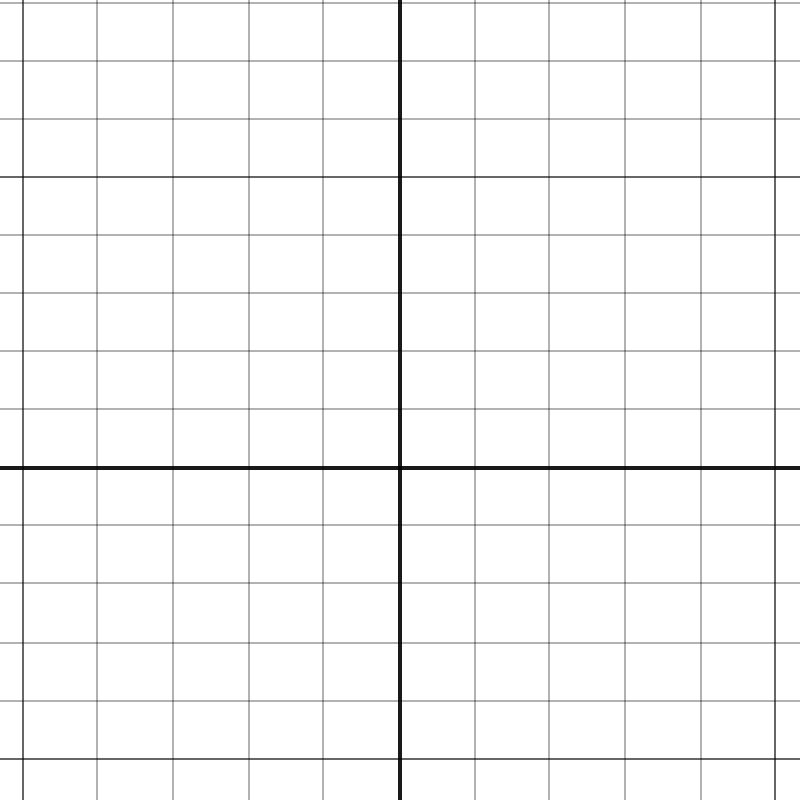
\includegraphics[alt={Blank graph paper for plotting the horizontal or vertical line described in the problem.}, width=1.25in]{105_graphpaper.jpg}
  
\item
  A vertical line that passes through the point $({2, -5})$. \\ \phantom{.}\hfill
  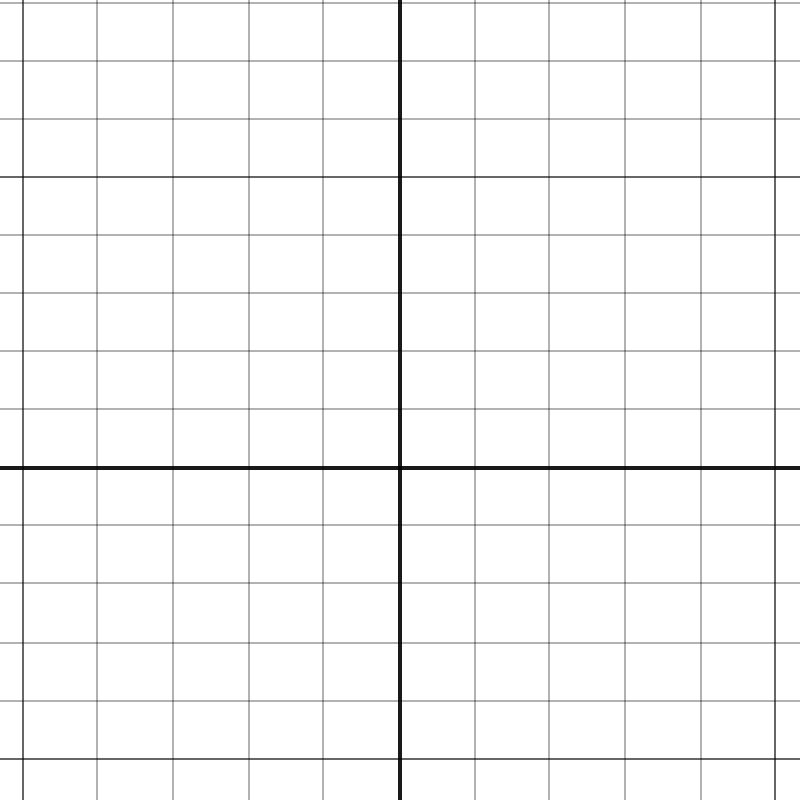
\includegraphics[alt={Blank graph paper for plotting the horizontal or vertical line described in the problem.}, width=1.25in]{105_graphpaper.jpg}
\end{enumerate}




\pagebreak


\defn{\dt{Parallel and Perpendicular Lines} \\
Given two linear equations $f(x)=m_1x +b$ and $g(x)=m_2x +b$. \\

\begin{itemize}
	\item The lines $f$ and $g$ are \dt{parallel} if the slopes are equal (or, if both lines are vertical). \\
	In other words, 
	\begin{center}
		The lines $f$ and $g$ will be parallel if \underline{\hskip2in} 
	\end{center}
	
	\item The lines $f$ and $g$ are \dt{perpendicular} if 
	\begin{center}
		$m_1m_2=-1$ or \underline{\hskip2in} 
	\end{center}
	
\end{itemize}

\vskip12pt 
}


\ex{Let $f(x) = \frac25 x -7$ with point $P(2,-3)$ not on the line. }
\begin{enumerate}
	\item Find a line parallel to $f$ that passes through the point $P$. 
	\vfill 
	
	\item Find a line parallel to $f$ that passes through the point $P$. 
	\vfill 
	
	\item Check your work by graphing all 3 lines on Desmos.com.
	
\end{enumerate}





\pagebreak


\ex{A line passes through the points $(-2, 6)$ and $(4, 5)$.  Find the equation of a perpendicular line that passes through the point $(4, 5)$.
}
\vfill 


\defn{\dt{Intersections of Lines} \\

If two lines are not parallel, then the graphs will intersect. \\
They will intersect at the point that satisfies \emph{both} equations. \\ 

To find this point when the equations are given as functions, \\ we can solve for an input value so that $f(x)=g(x)$.  \\

In other words, we can set the formulas for the lines \underline{equal}, \\
and \underline{solve} for the input that satisfies the equation.
\vskip12pt 
}


\ex{Find the intersection point of the lines $D(t)= 3t-4$ and $S(t)=5-t$.
}
\vfill 







\end{document}
